% Chapter 5

\chapter{SYSTEM DEVELOPMENT} % Write in your own chapter title

\section{Input and Output to System}
\subsection{Input}
Basic hand gestures are the input to the system. We have the following hand gestures \newline \newline 
1) Swipe left  \newline
2) Swipe right \newline
3) Swipe up \newline
4) Swipe down \newline
5) Circle 
\subsection{Output}
The output of the system is an appropriate response from the robot to the gesture.\newline
1) A swipe left gesture results in the robot moving to the left\newline
2) A swipe right results in the robot moving to the right\newline
3) A swipe up results in the robot moving forward\newline
4) A swipe down results in the robot moving backward\newline
5) A circle results in the robot moving in a circular manner\newline
\section{Input and Output for each module}
\subsection{Raspberry-pi controlled Robot}
\textbf{Input}\newline
The input to Raspberry Pi is the gesture packets from the internet.\newline
\textbf{Output}\newline
The output is the motion of the robot based on the Gestures.\newline
\textbf{Process}\newline
\textbf{Code for Robot Control}\newline
Forward Movement \newline
\begin{lstlisting}
def forward(tf): 
gpio.output(7,False)
gpio.output(11,True) 
gpio.output(13,True) 
gpio.output(15,False) 
time.sleep(tf)
gpio.cleanup()
\end{lstlisting} 
Backward Movement \newline
\begin{lstlisting}
def reverse(tf):
gpio.output(7,True)
gpio.output(11,False)
gpio.output(13,False)
gpio.output(15,True) 
time.sleep(tf) 
gpio.cleanup()

\end{lstlisting}


\subsection{Kinect-PC module for gesture recognition}
\textbf{Input}\newline
The input here is the gestures like swipe left, swipe right, swipe up, swipe down, the ability to control the mouse and drawing a circle. \newline
\textbf{Output}\newline
The output is the gesture packets. These are stored in the system, after the program is run.\newline
\textbf{Process}\newline
Swipe to Right
\begin{lstlisting}
{
if ((final vector.Y - initial vector.Y >maximum height) &&
(final vector.X - initial vector.X >0) &&
(swipe duration >minimum duration) &&
(swipe duration <maximum duration))
Swipe Right Gesture detected;
}
\end{lstlisting}
Swipe to Left
\begin{lstlisting}
{
if ((final vector.Y - initial vector.Y >maximum height) &&
(final vector.X - initial vector.X <0) &&
(swipe duration >minimum duration) &&
(swipe duration >maximum duration))
Swipe Left Gesture detected;
}
\end{lstlisting}
\subsection{Internet-Interfacing the Gesture and Voice Recognition Device with the Robot}
\textbf{Input}\newline
The input here is the gesture packets stored in the system. \newline
\textbf{Output}\newline
The output is the packets being transmitted over the internet through SSH to the robot, and the robot understanding each packet and performing the action\newline
\textbf{Process}\newline
Sample pseudo-code for SSH connection over C\#
\begin{lstlisting}
using (var client = new SshClient("hostnameOrIp", "username", "password"))
{
    client.Connect();
    client.RunCommand("etc/init.d/networking restart");
    client.Disconnect();
}
\end{lstlisting}


\section{Modules}
\subsection{Raspberry-pi controlled Robot}
Since the aim is to build a prototype, the emphasis is not on a specific task the robot should accomplish. Hence, a simplistic robot with basic motor functions is built. The robot can navigate in all directions i.e left, right, front and back; capable of turning and manoeuvring on its path. 
We make use of an L298N motor driver. A full h bridge is used because we need to run four motors. A half bridge runs only 2 motors and L298N is more powerful than L298D (half bridge). We have 200 RPM DC motors which can rotate clockwise and anticlockwise. The RPI (raspberry pi) is set up by installing the Raspbian OS (flavour of Linux) and we dedicate an 8GB SD card to it as fast and better processing will be required in the future. We chose 512 MB ram also for the same reason. The GPIO pin is set up and so is the corresponding package bundle for the RPI. The remote desktop server (Xbmc) and the SSH terminal is set up on the RPI. This is done so that the RPI can be remotely accessed via the DLink Wi-Fi adapter using the TP-Link wireless router. The Wi-Fi adapter is also installed with a powered USB hub because the RPI does not have enough power to directly handle a Wi-Fi adapter. This is set up and all the GPIO pins were connected to the motors. A corresponding python program is written to control the dc motors and rotate the wheels of the motor in the forward and backward directions. 
On completion, the program is modified to interface with the keyboard strokes by using the TKinter interface which identifies the keyboard strokes on press. Basic level of design includes communication of error free gesture signals to the computer which are subsequently forwarded through the Internet to the robot (raspberry-pi). At the first stage of development, primitive signals from the keyboard of the computer were successfully transmitted to the robot. These signals were correctly understood and the robot moved in the appropriate directions. For e.g on pressing A,W and D , the robot moved left, forward and right respectively. 
At the next stage of development, this was then connected to the laptop using the Microsoft remote desktop server by setting up a static IP in the RPI. The static IP is set up because of the constant change in IP every time it connects to the network. The static IP is used to remotely access the RPI and run the program on the laptop and use the laptop keys to move the robot. Directions like forward, backward, turn left, turn right, sharp left, sharp right have been programmed for specific key strokes. 
We are able to access the robot remotely from any location using mobile phone or pc. We have done this using VNC (virtual network controller) server and remote SSH (secure shell) connection. We first installed the VNC server and updated it. We then wrote a shell script that starts the VNC server as soon as the pi is turned on. We then configure the pi with a static IP address over the internet. Initially, the IP address was dynamic and it kept changing every time the pi went on the internet. We solved this problem by using dynamic DNS from no-ip.com. This helped us assign dynamic DNS to the robot which we can use anytime. The VNC server makes use of port 5901 and SSH using port 22. We have moved our robot from other locations in Chennai, Bangalore, Delhi and Nigeria. 
At the final stage of development, a 5 megapixel NO IR camera was attached to the RPI camera slot. This was then updated and upgraded and the Camera module in the RPI was enabled so that we can take photos and videos from the Camera. A web based application was then created to stream the video from the RPI to the webpage. This was done using the MP4 conversion to stream lesser number of bytes over the internet for continuous streaming of the videos. The IP address of the RPI was put in the web browser for the video to start streaming. The video module code was written in Python on the RPI and this code gets triggered immediately after the booting of the RPI in the shell script. Thus the video is enabled and continuous MP4 videos are streamed to the browser over the internet.


\begin{figure}[H]
  \centering
  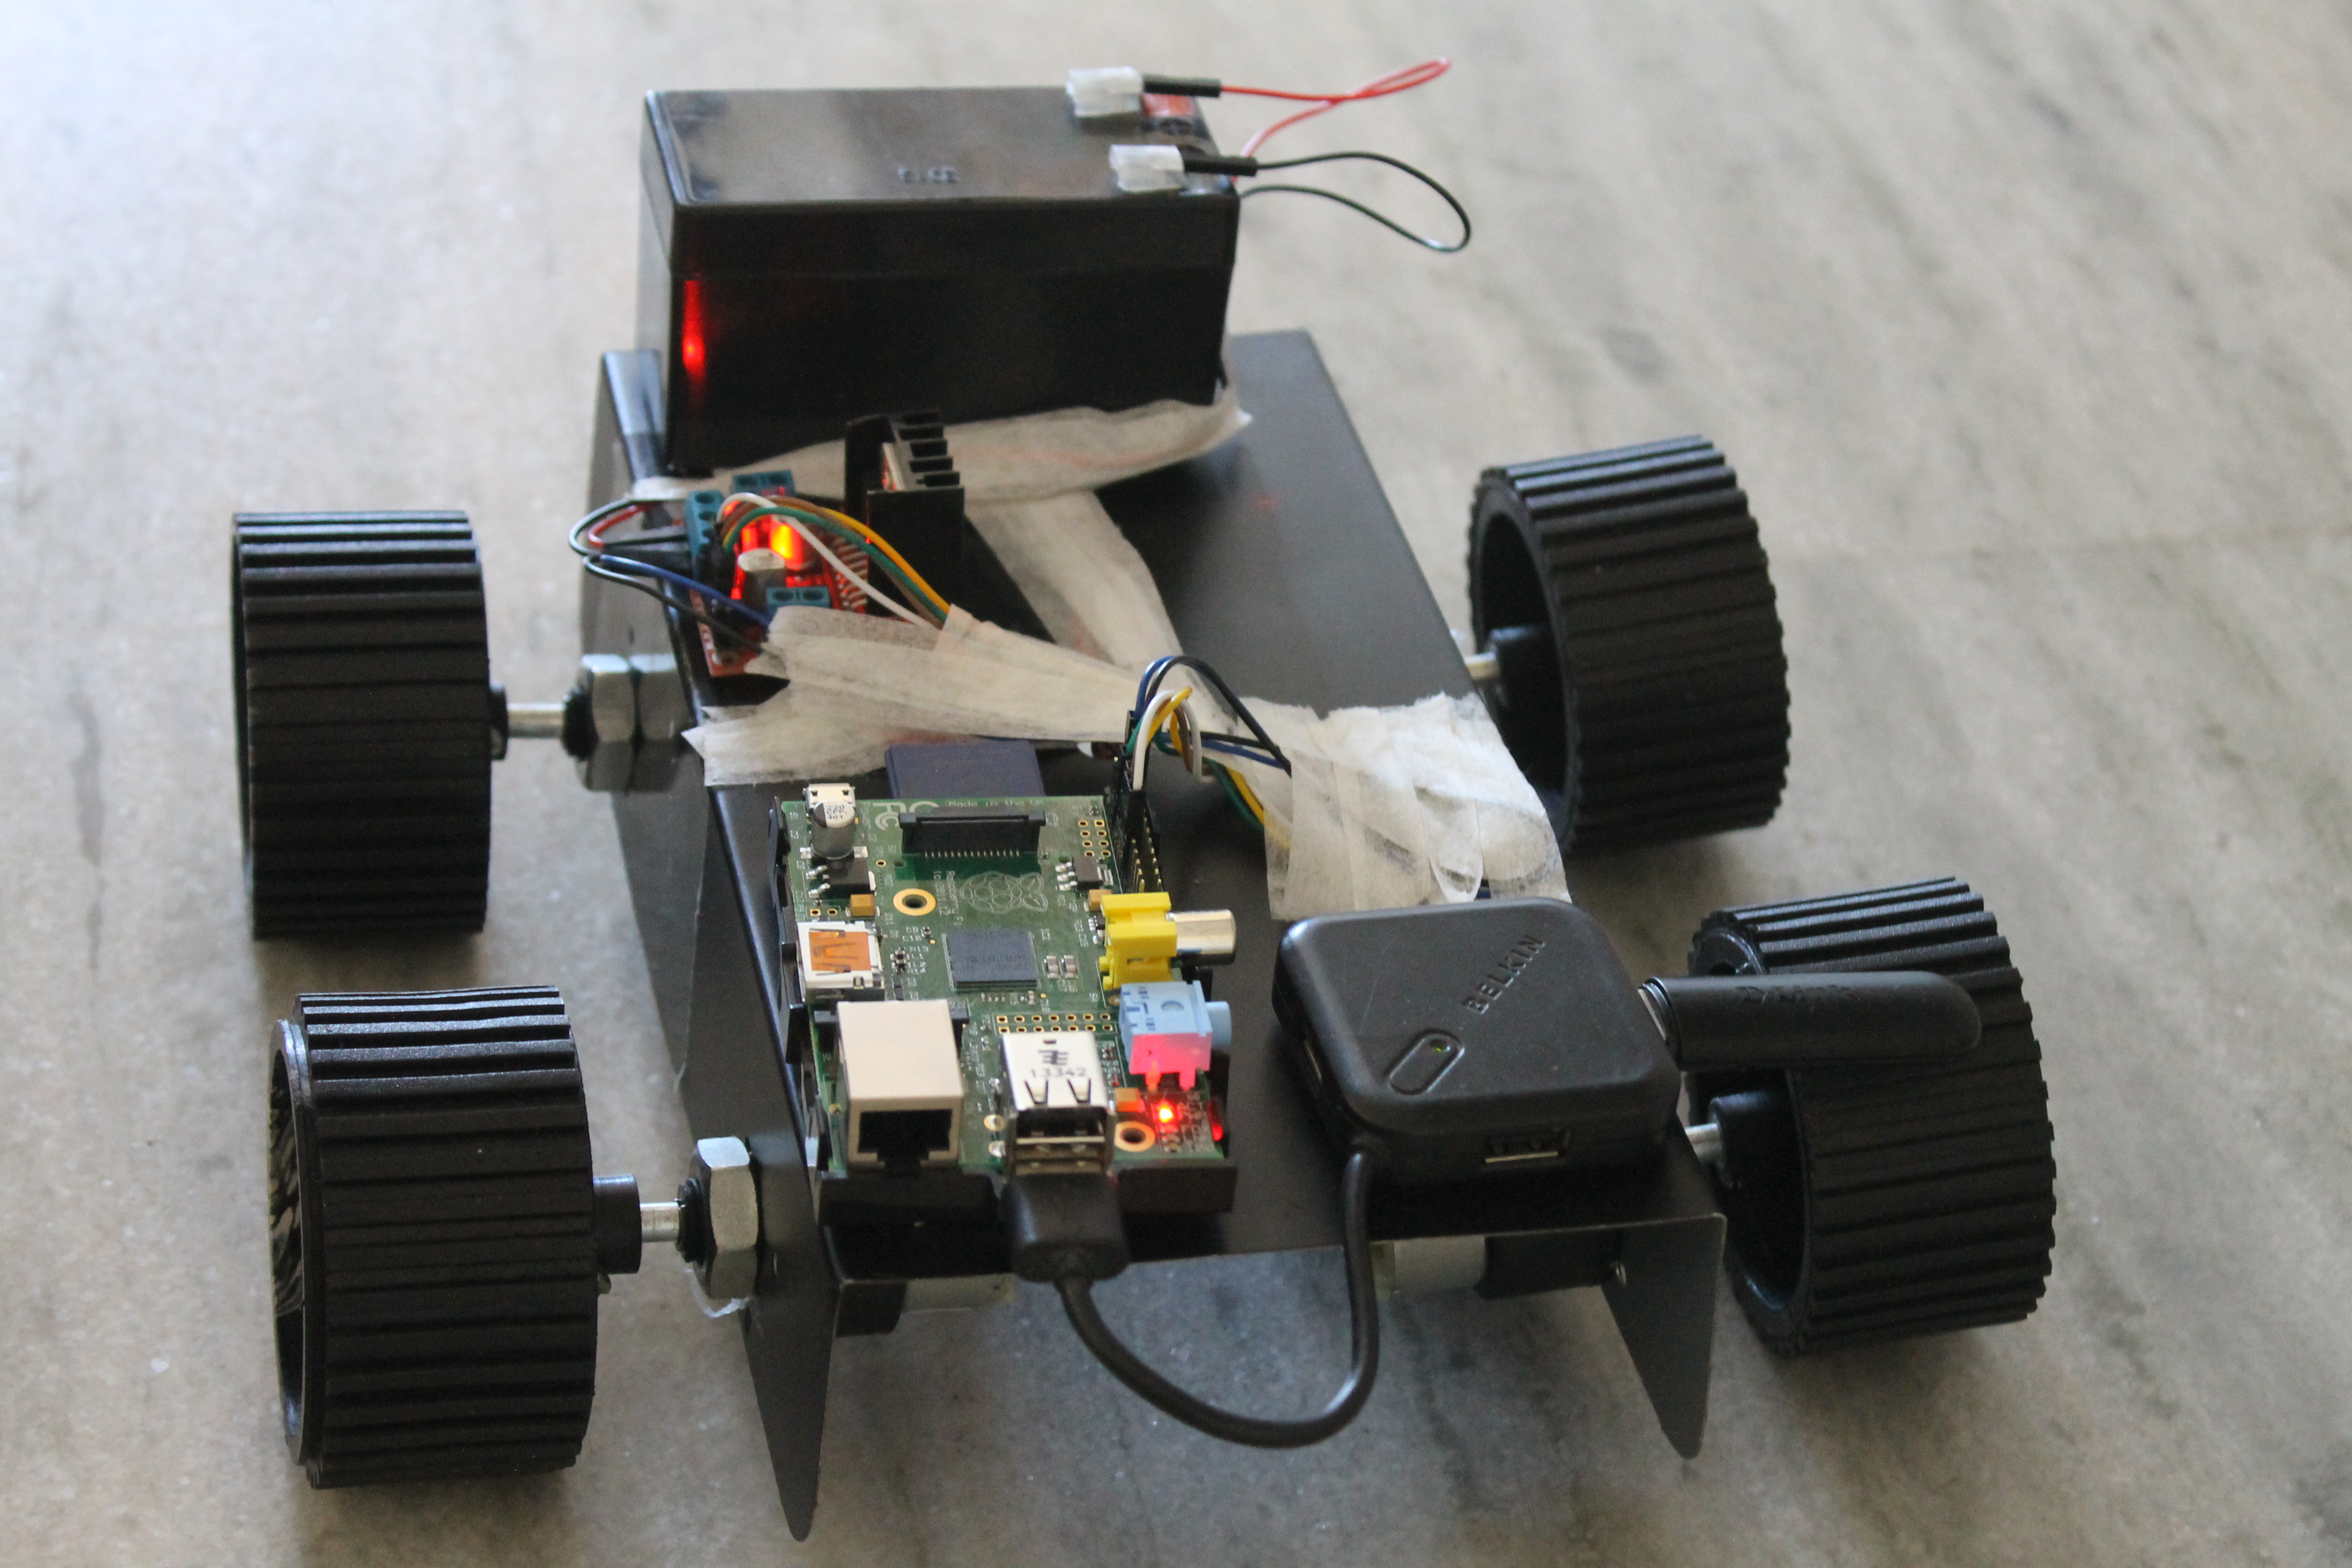
\includegraphics[width = 15cm, height = 11cm]{InitialRobot.jpg}
  \caption{The Preliminary Robot which could Only be Moved through Computer or Phone}
  \label{first robot}	
\end{figure}

\begin{figure}[H]
  \centering
  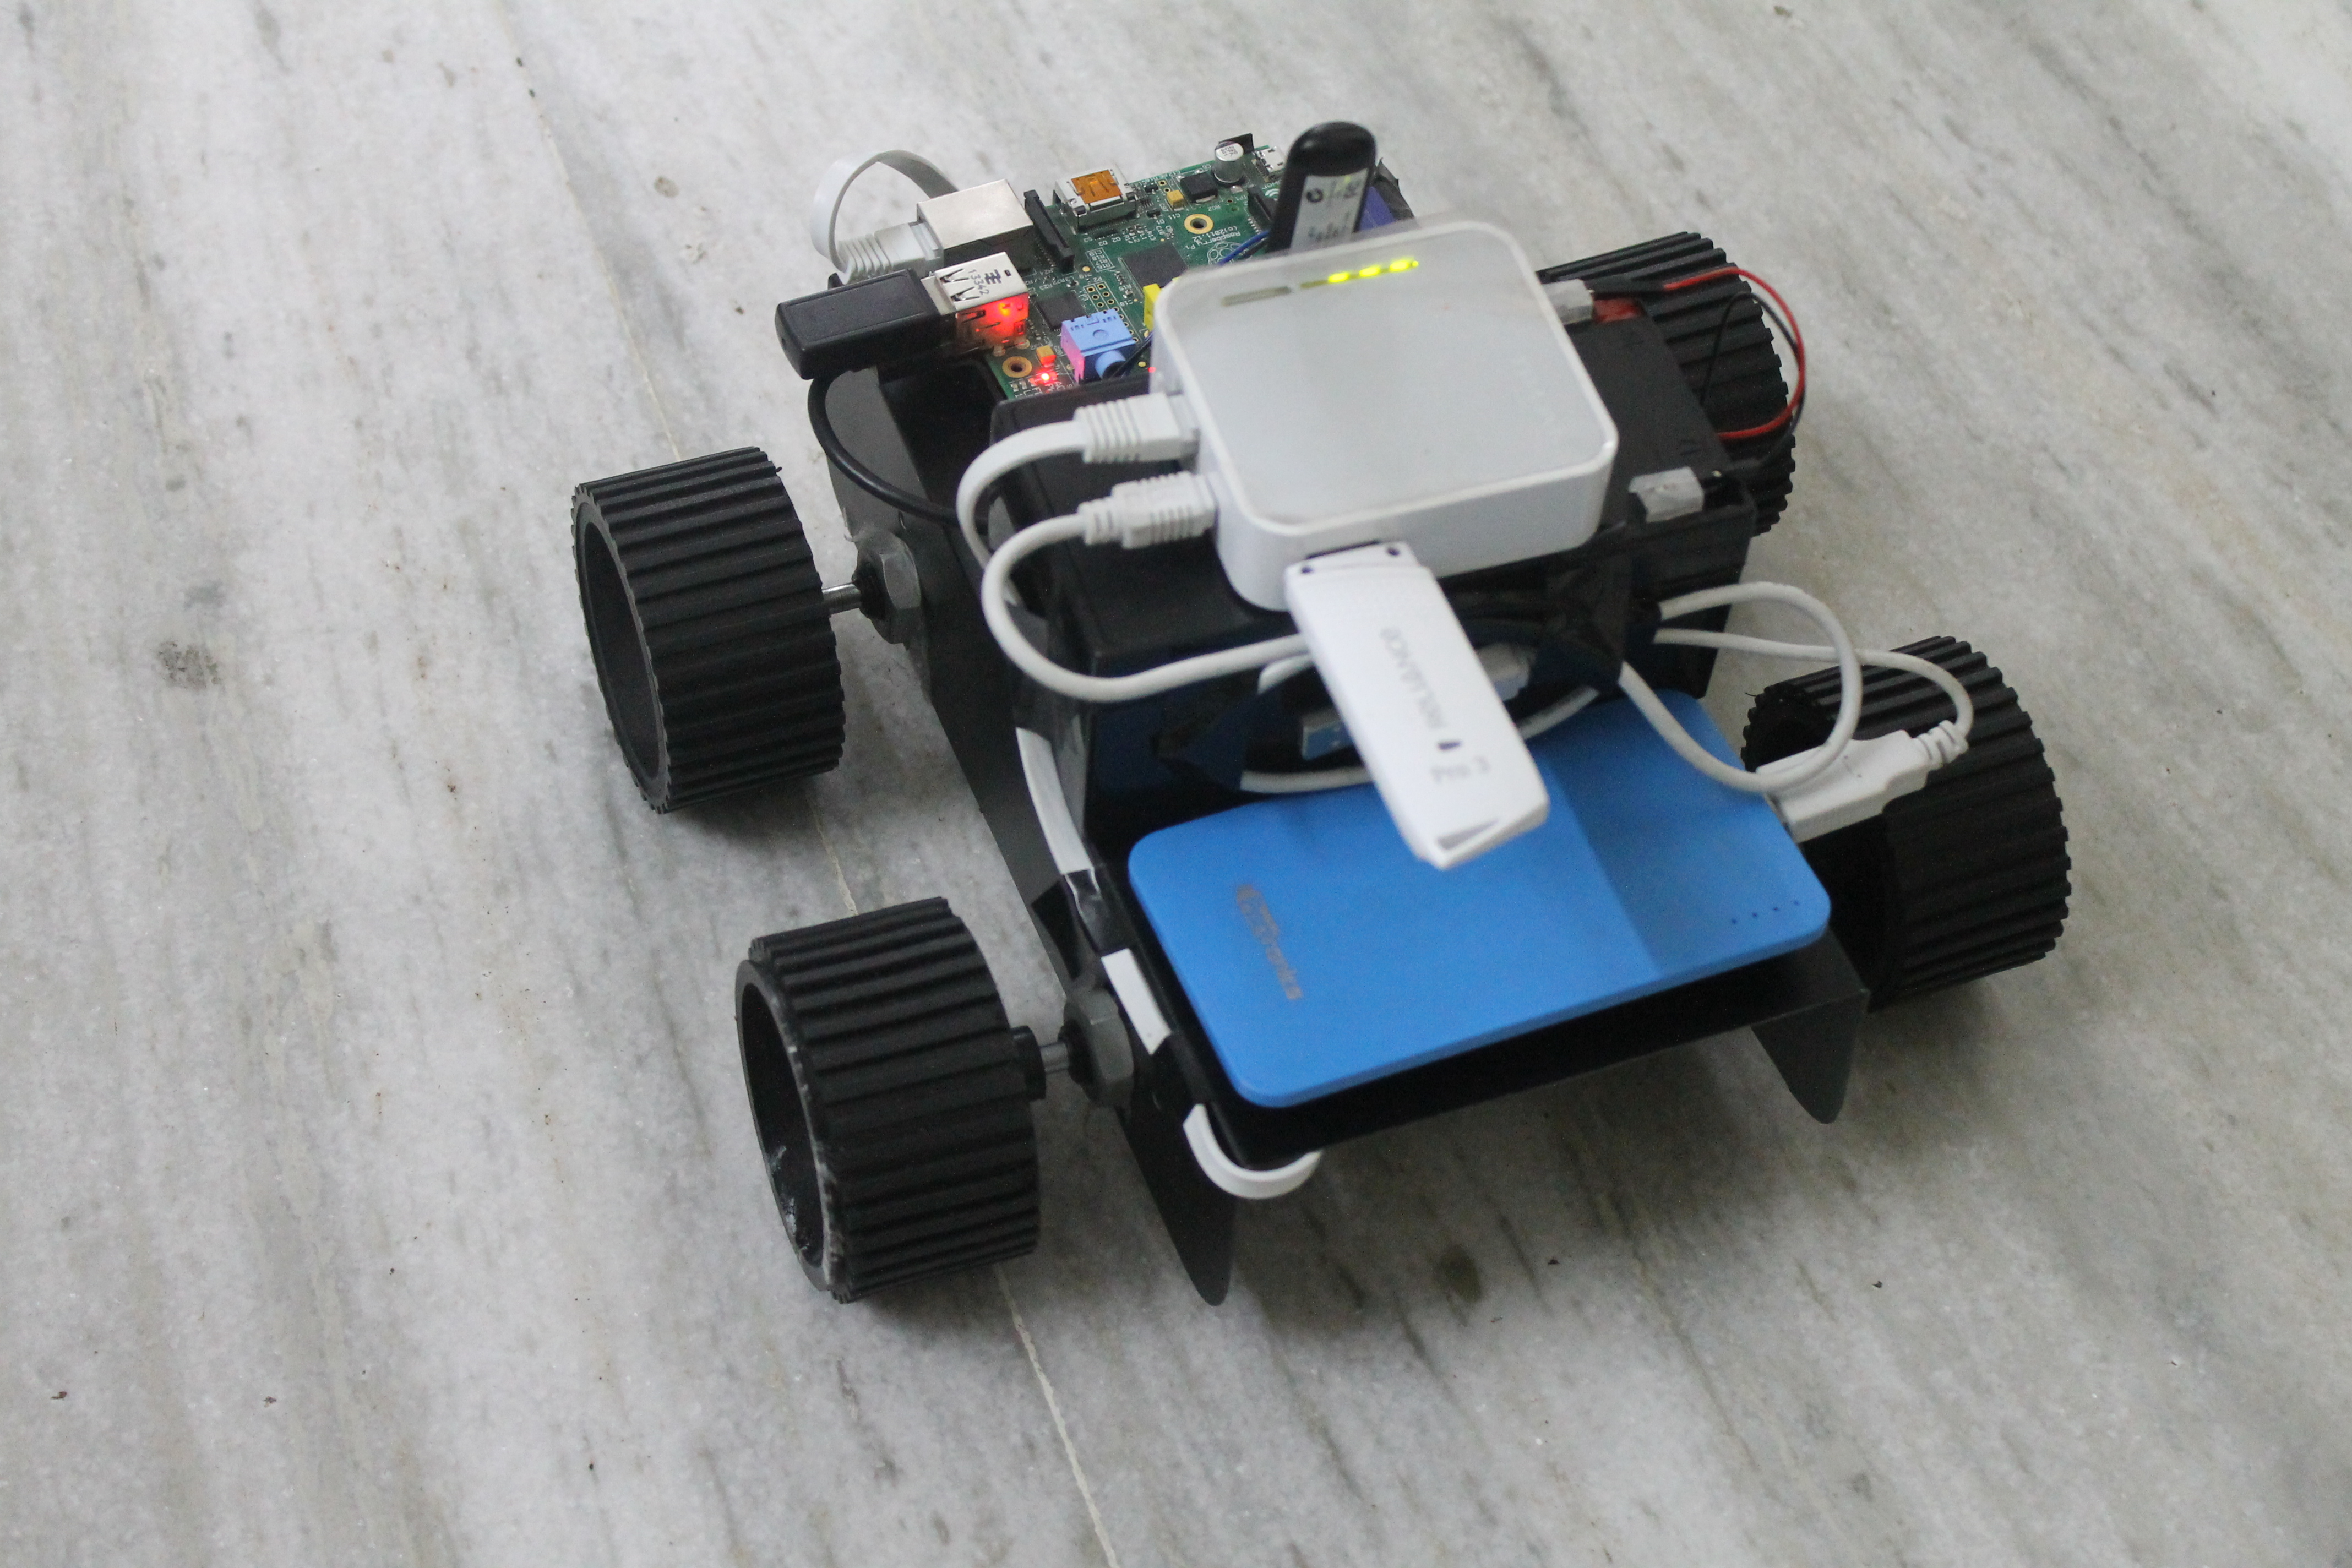
\includegraphics[width = 15cm, height = 11cm]{SecondRobot.jpg}
  \caption{The Fully Functional Robot without the Camera}
  \label{second robot}	
\end{figure}



\subsection{Kinect-PC module for gesture recognition}
In order to control the robot, we require a gesture and voice recognition device. The Microsoft Kinect for Windows is the best suited device for our requirements. To recognise gestures from the Kinect, we purchased the Microsoft Kinect and downloaded the Kinect for Windows Software Development Kit (SDK). The SDK provides the tools and APIs, both native and managed, that we need to develop Kinect-enabled applications for Microsoft Windows.
Developing Kinect-enabled applications is essentially the same as developing other Windows applications, except that the Kinect SDK provides support for the features of the Kinect, including colour images, depth images, audio input, and skeletal data. Programming the Kinect to recognise the gestures is done in C sharp programming language, in a .NET framework. We then plan to make use of open source softwares like OpenKinect which will help us to use the Kinect?s hardware with other devices. We have gone in a step-wise manner while recognizing the gestures. We have recognized basic gestures like swipe left and swipe right. In order to achieve that, we have written an algorithm that takes each and every point on the hand and checks for the constraints.
For the SwipeRight gesture, we will use constraints like:
\begin{verbatim}
1. Each new position should be to the right of the previous one
2. Each position must not exceed in height the first by more than a given distance (20 cm)
\end{verbatim}
Similarly, we program the SwipeLeft gesture with another algorithm. Some of the other constraints in our program are that, the swipe left and swipe right gestures only work for the right hand. Moreover, to recognize the gesture accurately, the person must stand at a distance of at least 4 feet. After recognizing basic gestures, we have moved on to complex gestures. We are able to control the movement of the mouse using our left hand. We can basically move the mouse any where on the screen. To click, we draw a circle using the right hand. To double click, we need to draw two such circles. Thus we have been successful in recognizing even complex gestures.

\begin{figure}[H]
  \centering
  \includegraphics[width = 15cm, height = 12cm]{SkeletalRecognition.jpg}
  \caption{Recognition of Skeleton using Kinect}
  \label{skeleton}	
\end{figure}

\begin{figure}[H]
  \centering
  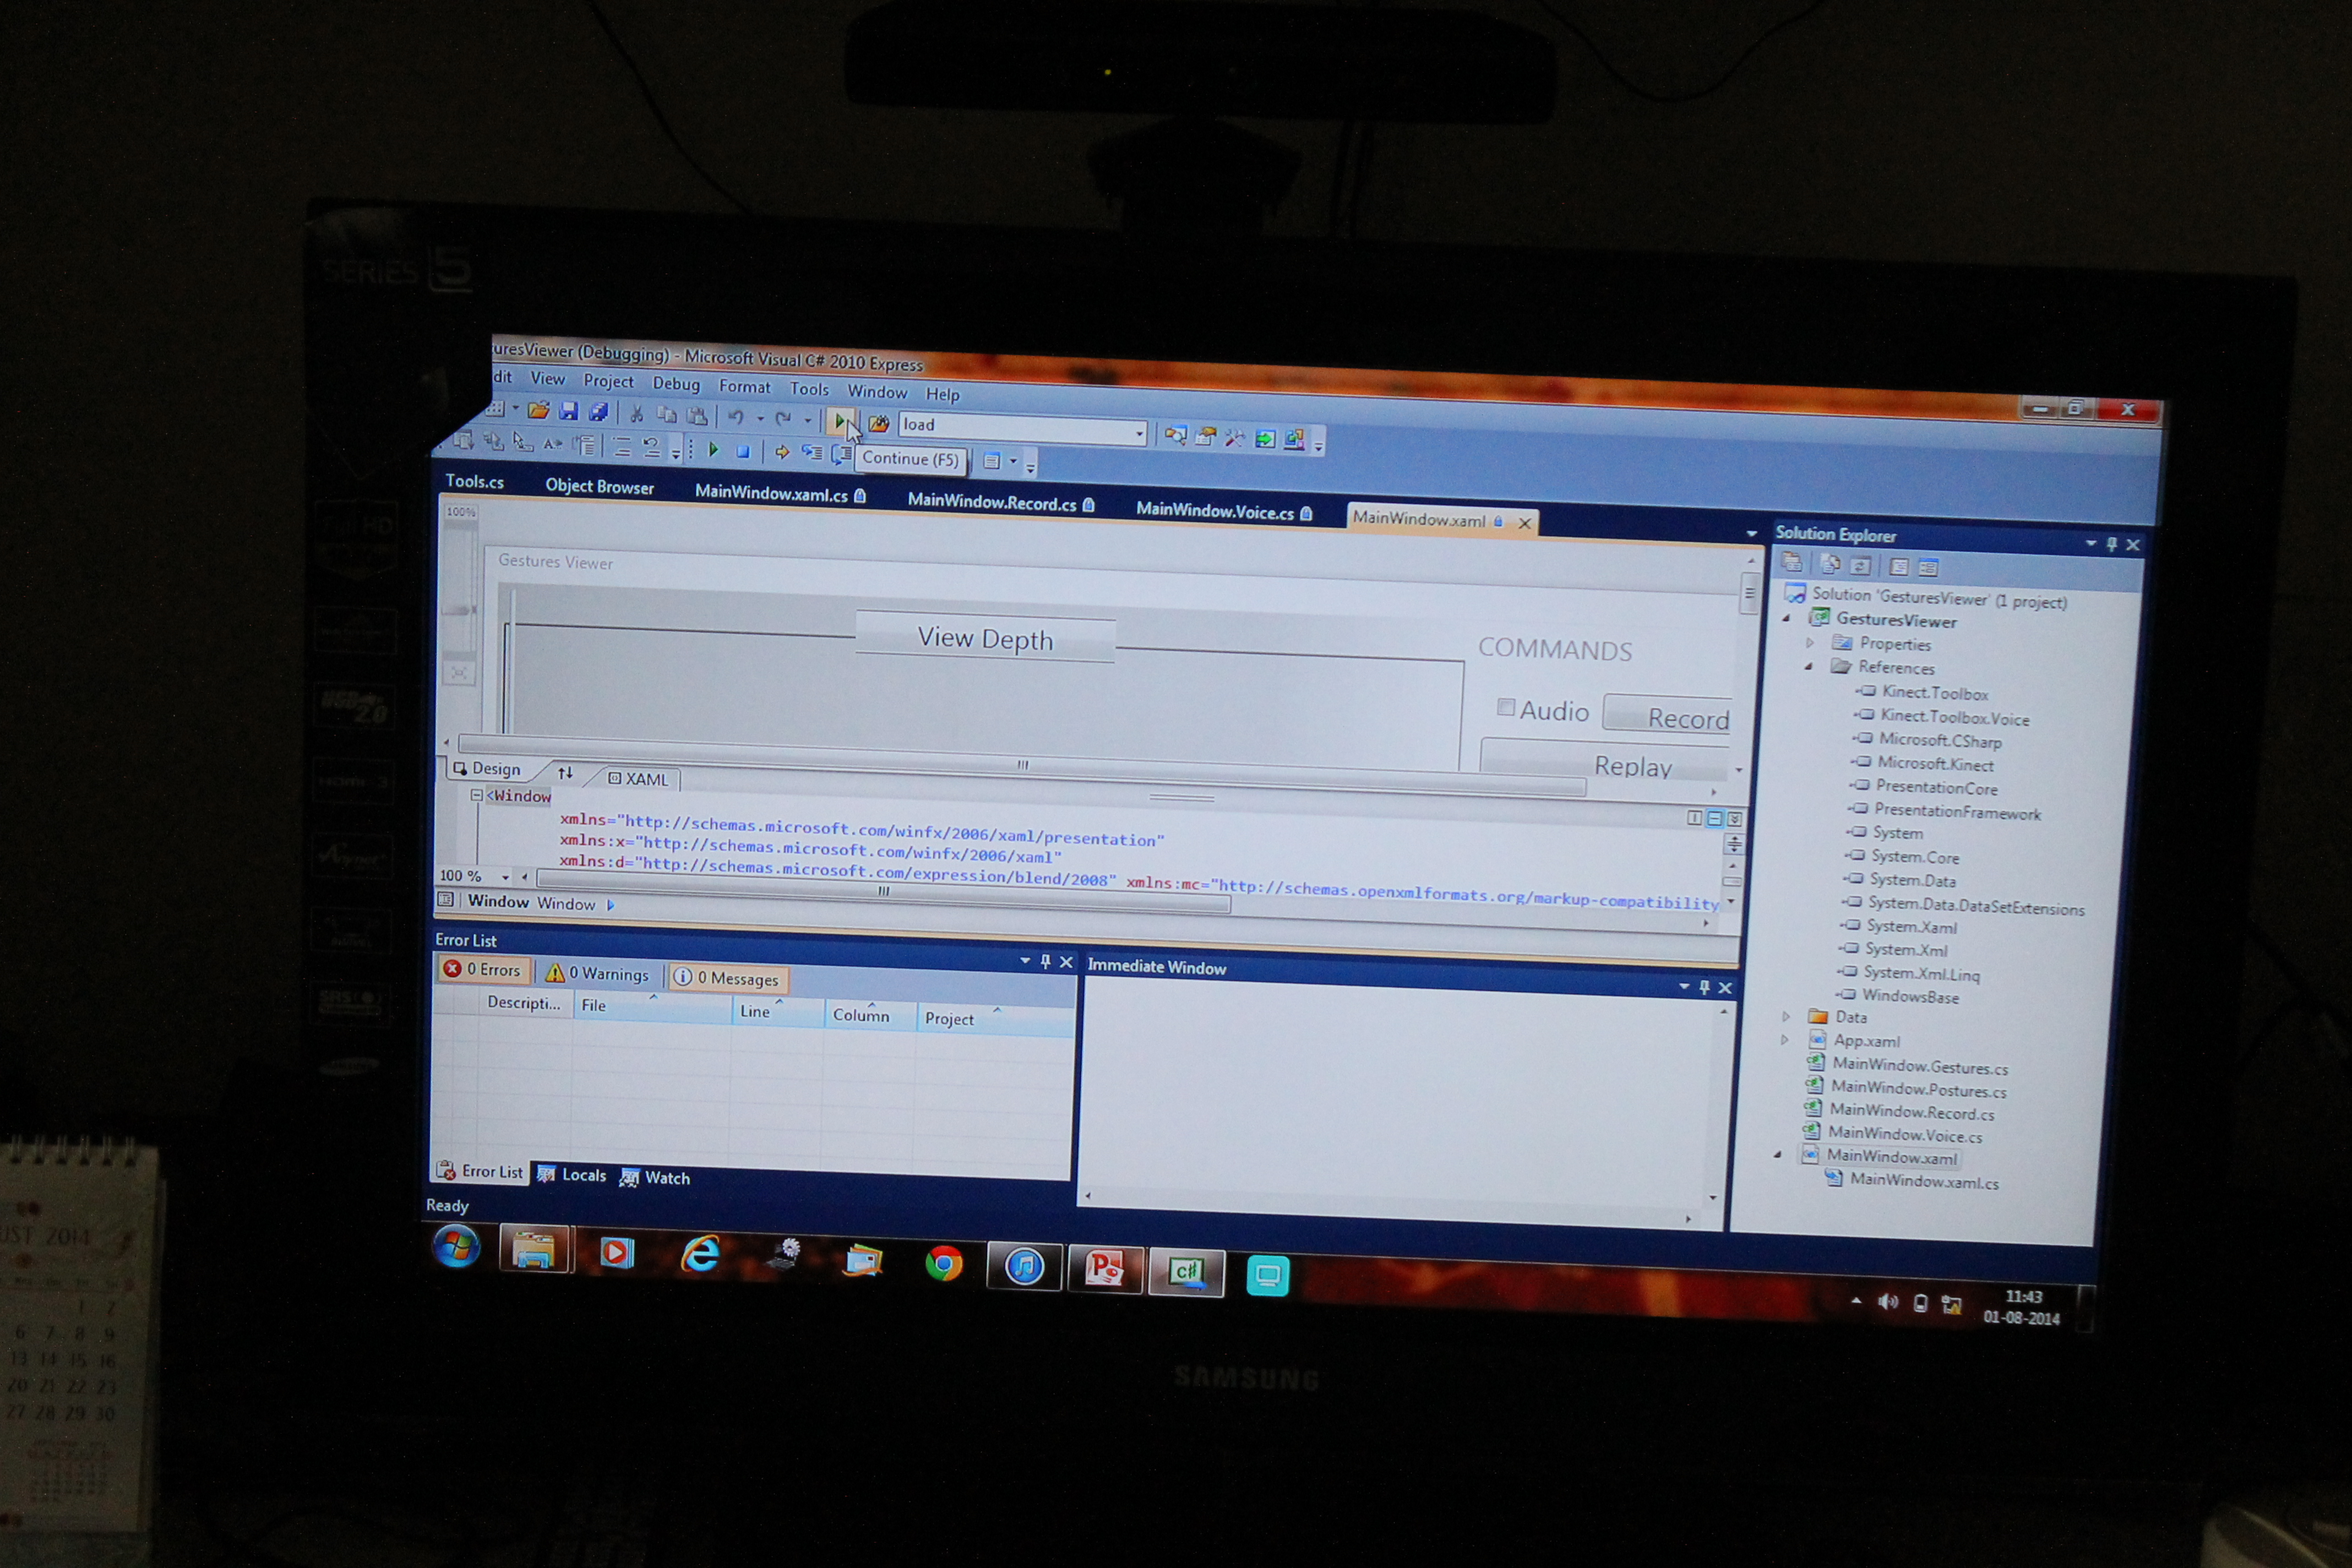
\includegraphics[width = 15cm, height = 12cm]{WPF.jpg}
  \caption{Programming for Kinect using C\# WPF Application}
  \label{WPF}	
\end{figure}

\subsection{Internet-Interfacing the Gesture and Voice Recognition Device with the Robot}
The connectivity between the raspberry-pi and the Kinect can be established through the internet or bluetooth. This particular arrangement of connecting the raspberry-pi over the internet and making it interact with the Kinect is an example of the internet of things and has not been exploited to its absolute potential. Interaction between the Arduino and the Kinect has been carried out through various platforms like the internet and bluetooth, but this has not been carried forward to the raspberry-pi. Due to various power requirements and other factors most attempts at such an integration have been unsuccessful. 
For every gesture performed by the user in front of the kinect, a separate code is written on robot that moves it according to the gesture. There are basically separate modules for each gesture.Once the gesture is recognized on the WPF(Windows Platform Framework) it is communicated using the SSH(Secure Shell Connection) over the internet to the robot. This is done using a noIP address, so that a static IP address is not required. Else, every time the robot connects to the internet, the IP address will change. Moreover, the SSH connection is persistent and open for all commands. Once the SSH connection has been established, we can perform all actions like SwipeRight, SwipeLeft etc and only upon program termination does the SSH connection close. This reduces time delay and improves performance. If the SSH connection was opened and closed for each individual gesture, it would be a serious bottleneck on the performance. Once the gesture packets reach the robot, it senses the command and executes the appropriate python program. Complex elliptical gestures like family of circles that make the robot rotate about itself are defined based on two simple previously defined gestures(swipe left immediately followed by a swipe right).
Thus we have been able to successfully interface a gesture recognition device(Microsoft Kinect) and a robot controller(Raspberry-Pi) over the internet. 


\section{Software Implementation Flow}

\begin{figure}[H]
  \centering
  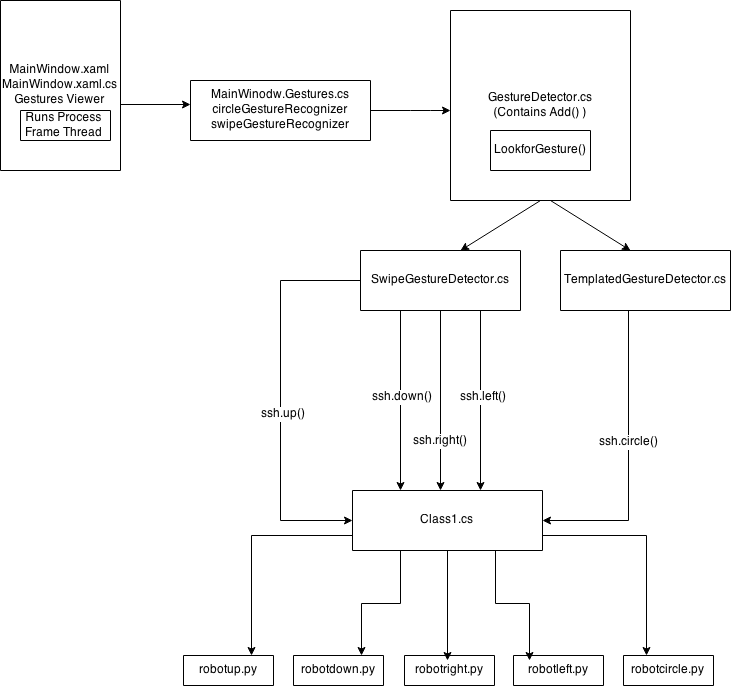
\includegraphics[width = 15cm, height = 12cm]{software.png}
  \caption{Software Flow Diagram}
  \label{Software Flow}	
\end{figure}

